\section{Method}
\label{sec:method}
\begin{figure*}[t]
\centering
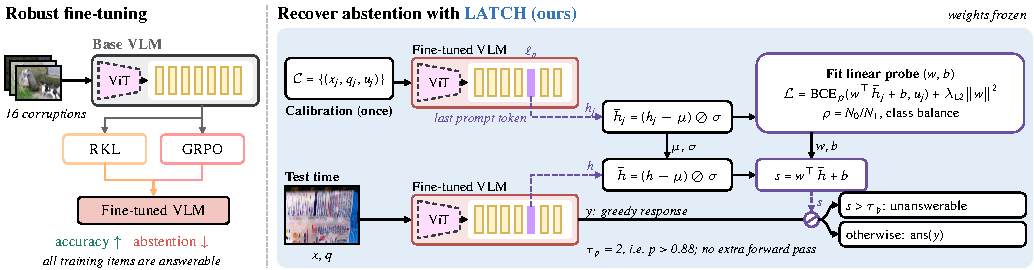
\includegraphics[width=\textwidth]{figures/method.pdf}
\caption{\textbf{Overview.} Robust fine-tuning (RKL or GRPO) raises accuracy but lowers
abstention. LATCH restores it with frozen weights: a latent check, fitted once per model on
a calibration set $\mathcal{C}$, replaces the answer by ``unanswerable'' when the probe
logit $s$ exceeds $\tau_{\mathrm{p}}$ ($P(\text{unanswerable}) > 0.88$). $(x, q)$: image and
question; $y$: response; $u$: answerability label ($u = 1$: unanswerable);
$\mathrm{BCE}_\rho$: binary cross-entropy that weights the $N_1$ unanswerable calibration
items by $\rho = N_0/N_1$, with $N_0$ answerable items. The two baselines are drawn in \cref{fig:supp_retrain,fig:supp_steer}.}
\label{fig:method}
\end{figure*}

Given a base VLM $\pi_0$, we make it robust to corruptions, locate what this does to its
abstention, and then repair it, which solves the problem of \cref{sec:problem}, in three
steps:
\ding{182}~We fine-tune $\pi_0$ on corrupted images with RKL or GRPO, which gives
$\pi_\theta$ (\cref{sec:method-ft}).
\ding{183}~We locate where abstention is lost, which tells us what an intervention can use:
a linear probe reads $u$ from the model's hidden state (\cref{eq:diagnose}), and a
reasoning transplant tests whether $\pi_\theta$ drops the refusal in its reasoning or in
its answer (\cref{sec:method-diagnose}).
\ding{184}~We recover abstention (\cref{eq:recover}) with three interventions $g$:
retraining on an unanswerable mix, LATCH, a latent check that turns the probe of
step~\ding{183} into a refusal rule, and activation steering
(\cref{sec:method-remedies}).

\subsection{Corruption-robust fine-tuning}
\label{sec:method-ft}

Both recipes train $\pi_\theta$ on its own sampled responses to the corrupted image
$\tilde{x}$. They differ only in what scores those responses: a teacher's token
distribution for RKL, a verifiable reward for GRPO.

\paragraph{On-policy reverse-KL distillation (RKL).}
Knowledge distillation trains a student to match a teacher's output distribution instead
of hard labels~\cite{hinton2015distilling}. On-policy
distillation~\cite{agarwal2024onpolicydistillationlanguagemodels} lets the student sample
its own responses and has the teacher score every token of them, so the student is
corrected on the prefixes it reaches itself rather than on the teacher's (exposure bias).
Here the student $\pi_\theta$ sees $\tilde{x}$, and a frozen teacher
$\pi_{\mathrm{teach}}$, a larger model of the same family, sees the clean image $x$. For
each question we sample $N_{\mathrm{roll}} = 2$ responses
$y \sim \pi_\theta(\cdot \mid \tilde{x}, q)$ and minimize the reverse KL at every position
$t \in \{1,\dots,T\}$:
\begin{equation}
\begin{aligned}
\mathcal{L}_{\mathrm{RKL}}(\theta) = \mathbb{E}\Big[\textstyle\sum_{t=1}^{T}
\mathrm{KL}\big(&\pi_\theta(\cdot \mid y_{<t}, \tilde{x}, q) \\
\,\big\|\,&\pi_{\mathrm{teach}}(\cdot \mid y_{<t}, x, q)\big)\Big],
\end{aligned}
\label{eq:rkl}
\end{equation}
with the expectation over $(x, \tilde{x}, q) \sim \mathcal{D}_{\mathrm{train}}$ and
$y \sim \pi_\theta(\cdot \mid \tilde{x}, q)$. Each term measures how far the student's
next-token distribution on $\tilde{x}$ is from the teacher's on $x$, after a prefix the
student wrote itself. Reverse KL is mode-seeking: the student concentrates on the
teacher's dominant continuations rather than covering all of them~\cite{gu2024minillm}. We
estimate each term from the sampled token, as a policy gradient with advantage
$A_t = \log \pi_{\mathrm{teach}}(y_t \mid \cdot) - \log \pi_\theta(y_t \mid \cdot)$.
RKL needs
no gold answers, only teacher forward passes.

\paragraph{Group Relative Policy Optimization (GRPO).}
GRPO~\cite{shao2024deepseekmath} replaces the teacher with a verifiable reward and PPO's
value network with a group baseline, and it sees only $\tilde{x}$. For each question it
samples $G = 8$ responses $y^{(i)} \sim \pi_{\theta_{\mathrm{old}}}(\cdot \mid \tilde{x}, q)$,
$i \in \{1,\dots,G\}$, from the policy before the update, and scores each as
\begin{equation}
r_i = \mathds{1}\!\left[\mathrm{fmt}_i \wedge \mathrm{ans}(y^{(i)}) = a^\star\right]
      + w_{\mathrm{fmt}}\, \mathrm{fmt}_i,
\label{eq:reward}
\end{equation}
where $\mathrm{fmt}_i \in \{0,1\}$ is $1$ if $y^{(i)}$ has exactly one \texttt{<answer>}
block and ends right after it, $w_{\mathrm{fmt}} = 0.1$, and $a^\star$ is the GQA gold
answer (exact match). For
example, a well-formed response with the gold answer earns $r_i = 1.1$, a well-formed wrong
answer $0.1$, and a response cut off before its \texttt{<answer>} block $0$. Advantages are
standardized within the group,
\begin{equation}
\hat{A}_i = \frac{r_i - \mathrm{mean}(r)}{\mathrm{std}(r) + \epsilon_{\mathrm{std}}},
\label{eq:adv}
\end{equation}
and the policy maximizes the clipped surrogate with a KL anchor to the base model:
\begin{equation}
\begin{aligned}
\mathcal{J}_{\mathrm{GRPO}}(\theta) = \mathbb{E}\Big[
&\tfrac{1}{\sum_i |y^{(i)}|}\textstyle\sum_{i,t}
\min\!\big(\rho_{i,t}\hat{A}_i,\, \bar\rho_{i,t}\hat{A}_i\big) \\
&- \beta\,\mathrm{KL}(\pi_\theta \,\|\, \pi_0)\Big].
\end{aligned}
\label{eq:grpo}
\end{equation}
Here $i$ ranges over the group and $t$ over the tokens of $y^{(i)}$,
$\rho_{i,t} = \pi_\theta(y^{(i)}_t \mid \tilde{x}, q, y^{(i)}_{<t}) /
\pi_{\theta_{\mathrm{old}}}(y^{(i)}_t \mid \tilde{x}, q, y^{(i)}_{<t})$ is the ratio of the
current to the sampling policy, $\bar\rho_{i,t} = \mathrm{clip}(\rho_{i,t},
1 - \epsilon_{\mathrm{clip}}, 1 + \epsilon_{\mathrm{clip}})$, $\epsilon_{\mathrm{clip}} = 0.2$,
$\epsilon_{\mathrm{std}} = 10^{-6}$ and $\beta = 0.04$; the token mean is taken over all
groups of an optimizer step. Because every training item has $u = 0$, a well-formed refusal
scores like any wrong answer ($r_i = 0.1$), and its advantage is negative whenever another
response in its group is correct: no term of \cref{eq:reward,eq:grpo} ever rewards
abstaining.

\subsection{Locating the loss}
\label{sec:method-diagnose}

We next ask where the refusal is lost: in the representation of answerability, in the
reasoning, or in the answer.

\paragraph{Answerability probe.}
For a model $\pi$ and decoder layer $\ell \in \{1,\dots,L\}$, one prefill gives the
residual-stream state $h^{(\ell)}_{\pi}(x,q) \in \mathbb{R}^{d}$ at the last prompt token,
the position just before the response begins. We standardize each of its $d$ features,
$\bar{h} = (h^{(\ell)}_{\pi}(x,q) - \mu) \oslash \sigma$ with $\oslash$ element-wise
division, by the mean $\mu$ and standard deviation $\sigma$ over a labeled calibration set
$\mathcal{C} = \{(x_j, q_j, u_j)\}_{j=1}^{N_{\mathcal{C}}}$, so that one L2 strength
penalizes all features on the same scale. We then fit a class-balanced, L2-regularized
logistic regression
\begin{equation}
p_\ell(u = 1 \mid x, q) = \mathrm{sigmoid}\big(w^\top \bar{h} + b\big),
\label{eq:probe}
\end{equation}
one per model and layer, on that model's own states; class balancing offsets the unequal
class sizes of $\mathcal{C}$. The AUROC of the logit $w^\top \bar{h} + b$ on held-out
items, $\mathrm{AUROC}_\ell(\pi) \in [0,1]$, measures how well layer $\ell$ of $\pi$ encodes
$u$; the same probe fitted on shuffled labels gives its chance floor. We say the probe
\emph{flags} an input when the logit exceeds $0$. Because the probe reads the state from
which the response starts, it tests whether
\begin{equation}
\begin{gathered}
\mathrm{AUROC}_\ell(\pi_\theta) \approx \mathrm{AUROC}_\ell(\pi_0) \\
\text{while}\ \
\mathrm{CR}(\pi_\theta;\mathcal{D}_{\mathrm{U}}) < \mathrm{CR}(\pi_0;\mathcal{D}_{\mathrm{U}}),
\end{gathered}
\label{eq:diagnose}
\end{equation}
\ie whether $\pi_\theta$ still encodes that the input is unanswerable when it begins to
answer. If so, the failure is behavioral rather than representational (RQ1), and an
intervention can use the signal that survives.

\paragraph{Reasoning transplant.}
A refusal can be lost in the reasoning, which never concludes that the image is
insufficient, or in the answer, which ignores reasoning that does. For example, on a blurry VizWiz photo
of jellybeans the RKL response lists flavors it cannot see, a reasoning-side failure, while
on \cref{fig:teaser}B the GRPO response states that the text ``cannot be deciphered with
certainty'' and still gives $\mathrm{ans}(y) = $ ``3232'', an answer-side failure. To separate the two at scale, we
take the unanswerable items that $\pi_\theta$ answered and $\pi_0$ refused, prefill
$\pi_\theta$ with $(x, q)$ followed by $\pi_0$'s response up to and including
\texttt{<answer>}, and record whether $\pi_\theta$'s answer is a refusal. If $\pi_\theta$
now refuses, its answer step follows a ``can't-tell'' chain, so its failure is that its own
reasoning never produces one; if it still answers, its answer step overrides the reasoning. Further details on this is given in \cref{sec:rq2}

\subsection{Recovering abstention}
\label{sec:method-remedies}

We finally ask how to bring the refusal back without giving up the gains of
step~\ding{182}. Each remedy is an intervention $g$ in \cref{eq:recover}: the first changes
the training data, and the other two keep $\theta$ fixed and act at inference. On the
captcha question of \cref{fig:teaser}B, the mix makes a refusal the trained target for
images corrupted past recognition, LATCH replaces ``3232'' by a refusal when the
probe flags $(x,q)$, and steering moves the hidden states of $\pi_\theta$ toward those of
$\pi_0$ while it writes.

\paragraph{Unanswerable mix.}
The first remedy asks whether abstention was lost simply because the training signal never
contained it. We retrain $\pi_0$ from scratch with the same recipe and budget on a mix in
which $10\%$ of the questions are unanswerable: GQA images corrupted far past recognition,
with $a^\star = $ ``unanswerable'' (Destroyed-GQA, \cref{sec:setup}; see \cref{fig:supp_retrain}). Abstaining is then
imitated (RKL, whose teacher sees the same destroyed image) or rewarded (GRPO, where a
well-formed refusal on these items now earns $r_i = 1.1$ in \cref{eq:reward}).

\begin{algorithm}[t]
\caption{\textbf{LATCH: one linear read of the prompt replaces an answer by a
refusal.} Lines 1--3 run once per model; lines 4--8 add no forward pass.}
\label{alg:latch}
\begin{algorithmic}[1]
\Require model $\pi$, layer $\ell_{\mathrm{p}}$, calibration set
  $\mathcal{C} = \{(x_j, q_j, u_j)\}$, L2 strength $\lambda_{\mathrm{L2}}$, cutoff
  $\tau_{\mathrm{p}}$
\State $h_j \gets h^{(\ell_{\mathrm{p}})}_{\pi}(x_j, q_j)$ for every
  $j$ \Comment{prefill only}
\State $\mu, \sigma \gets$ mean and std.\ of $\{h_j\}$;
  $\bar{h}_j \gets (h_j - \mu) \oslash \sigma$
\State $(w, b) \gets$ fit \cref{eq:probe} to $\{(\bar{h}_j, u_j)\}$, class-balanced, L2
  strength $\lambda_{\mathrm{L2}}$
\State On a test input $(x, q)$: prefill and read
  $\bar{h} \gets (h^{(\ell_{\mathrm{p}})}_{\pi}(x, q) - \mu) \oslash \sigma$
\State $y \gets$ greedy response of $\pi(\cdot \mid x, q)$ \Comment{reuses the prefill}
\If{$w^\top \bar{h} + b > \tau_{\mathrm{p}}$}
  \State \Return ``unanswerable''
\EndIf
\State \Return $\mathrm{ans}(y)$
\end{algorithmic}
\end{algorithm}

\paragraph{LATCH (LATent CHeck).}
The probe of \cref{sec:method-diagnose} still reads $u$ after fine-tuning (\cref{sec:rq1}),
so the second remedy acts on it directly (\cref{fig:method,alg:latch}). Lines~1--3 fit that probe at a
single layer $\ell_{\mathrm{p}}$, once per model and on that model's own states. Lines~4--5
run the model unchanged and reuse its prefill for the probe. Lines~6--7 replace the answer by
a refusal when the probe logit exceeds $\tau_{\mathrm{p}}$; line~8 otherwise returns the
model's own answer. Thus LATCH changes $\mathrm{ans}(y)$ only on inputs it flags, so
the robustness gained on answerable inputs is kept wherever it does not fire, and
$\tau_{\mathrm{p}}$ sets the trade-off between $\mathrm{CR}$ and $\mathrm{UR}$ in
\cref{eq:recover}.

\begin{algorithm}[t]
\caption{\textbf{Contrastive activation steering pushes the fine-tuned model back toward
the base model's refusal.} Shown for the image-contrast vector; the no-image vector
changes lines 1--3 (see text). The weights are never modified.}
\label{alg:steer}
\begin{algorithmic}[1]
\Require base $\pi_0$, fine-tuned $\pi_\theta$, pool $\mathcal{P}$ of unanswerable
  VizWiz-train items, layer $\ell_{\mathrm{s}}$, scale $\alpha$, gate threshold
  $\tau_{\mathrm{H}}$ ($\tau_{\mathrm{H}} < 0$: always on)
\State $\mathcal{S} \gets \{(x, q) \in \mathcal{P} : \mathrm{ref}(y_0) = 1,\
  \mathrm{ref}(y_\theta) = 0\}$, with $y_0, y_\theta$ the greedy responses of
  $\pi_0, \pi_\theta$
\State For each $(x, q) \in \mathcal{S}$, run $(x, q, y_\theta)$ through both models; collect
  $h^{(\ell_{\mathrm{s}})}_{0,t} - h^{(\ell_{\mathrm{s}})}_{\theta,t}$ at every response
  position $t$
\State $v \gets$ mean of the collected differences, $v \in \mathbb{R}^{d}$
\State On a test input, generate from $\pi_\theta$; at each decoding step $t$:
\If{$\tau_{\mathrm{H}} < 0$ \textbf{or} $H_{t-1} > \tau_{\mathrm{H}}$}
  \State $h^{(\ell_{\mathrm{s}})}_{\theta,t} \gets h^{(\ell_{\mathrm{s}})}_{\theta,t} + \alpha v$
\EndIf
\end{algorithmic}
\end{algorithm}

\paragraph{Activation steering.}
The third remedy also uses the intact representation, but changes the hidden states instead
of reading them (\cref{alg:steer,fig:supp_steer}). We write $h^{(\ell)}_{0,t}$ and $h^{(\ell)}_{\theta,t}$
for the layer-$\ell$ states of $\pi_0$ and $\pi_\theta$ at response position $t$. Line~1
keeps exactly the calibration questions on which fine-tuning broke abstention, so that the
vector captures what fine-tuning changed rather than refusal in general. Line~2 feeds the
same text (image, question and $\pi_\theta$'s own response) through both models, so that the
difference reflects the two models rather than two inputs. Line~3 averages over every
response position of every selected question. Thus $v \in \mathbb{R}^{d}$ points from the
fine-tuned model's over-confident state toward the base model's ``this image does not
support an answer'' state. The \emph{no-image} vector targets a missing image instead: it
pairs questions asked without their image on which $\pi_0$ refuses and $\pi_\theta$
answers, runs the question followed by the base refusal and the question followed by the
fine-tuned answer through $\pi_\theta$, and averages the difference of the
response-averaged states. Lines~4--6 add $\alpha v$ to the residual stream at layer
$\ell_{\mathrm{s}}$ on generated tokens only, upstream of the layers where answerability is
most decodable, so that the push lands before the tokens that commit to an answer. The
optional gate (line~5) steers only after uncertain steps, where the entropy
$H_{t-1} = -\sum_{z \in \mathcal{V}} p_{t-1}(z) \log p_{t-1}(z)$ of the previous
next-token distribution of $\pi_\theta$ exceeds $\tau_{\mathrm{H}}$; it uses step $t-1$
because the distribution at step $t$ depends on the push itself. We gate RKL, whose failure
lies in its reasoning (\cref{sec:rq2}), so that the push corrects confused steps and leaves
fluent ones alone; GRPO's failure is a uniform answer-level shortcut, so its push is always
on. All calibration data come from training splits with no evaluation overlap.
